\documentclass[notitlepage]{article}
\usepackage[utf8]{inputenc} 
\usepackage{geometry} 		
\usepackage{chngcntr}
\usepackage{amsmath} 			
\usepackage{amssymb}			
\usepackage{mathtools}		
\usepackage{comment} 			
\usepackage{mdframed}
\usepackage{hyperref}			
\usepackage{xcolor}				
\usepackage{fancyhdr}			
\usepackage{listings}			
\usepackage{color}				
\usepackage{tikz}	
\usepackage{tasks}			
\usepackage{exsheets}		
\usepackage{array}			
\usepackage{empheq}
\usepackage{caption}
\usepackage{pdfpages}
\usepackage{tabularx}

\geometry{ 						%Format titlepage (interrupted by newgeometry)
	a4paper,
	total={170mm,257mm}%,
	%left=0mm,
	%top=0mm,
}

%START DEFINE YOUR VARIABLES HERE

\newcommand{\documentName}{User Manual}
\newcommand{\projectName}{Label Refinement by Behavioral Similarity}

%END DEFINE YOUR VARIABLES HERE

\title{%
	\documentName\text{ } \\
  \large \projectName\text{ } \\
  }

\author{
	\large \underline{Document owners:}\\ 
	Bianka Bakullari\\
	\texttt{}
	Christopher Beine\\
	\texttt{}
	Nicole Ventsch\\
	\texttt{}
	Juan Garza\\
	\texttt{}
}

\date{\small{Last edited: \today}}

\pagestyle{fancy}
\fancyhf{}
\rhead{}
\lhead{\documentName\space-\space\projectName}

\makeatletter					%Prefix to add ToC to titlepage
\newcommand*{\toccontents}{\@starttoc{toc}}
\renewcommand*\contentsname{}
\makeatother
                  

\begin{document}

\begin{titlepage}
\clearpage\maketitle			%Clear title page
\thispagestyle{fancy}
\tableofcontents
\end{titlepage}

\rfoot{\thepage}				%Start printing page-numbers, after title page.

\newgeometry{ 					%Default page formatting on-going #1
	total={170mm,257mm},
	left=20mm,
	top=25mm,
    bottom=30mm					%Causes warning
}

%\begin{flushleft}				%Default page formatting on-going #2

\section{Overview}

Many processes involve carrying out an action multiple times. 
An example for this would be an online shop in which you first have to pay a registration fee before ordering an item and paying it. 
This process contains the event “payment" twice, but in different contexts, so that the payments are actually two different tasks. 
When analysing processes behind event logs, each event appearing in the log has a certain label as its \textit{activity name}, so if both tasks above had the label “payment", the process discovery algorithms would treat them as the same task, yielding models which contain loops. 
However, these loops do not match the actual process and make the model imprecise.
This could be avoided if the tasks above were assigned different labels, e.g: "payment1" and "payment2".
Manipulating the event log by refinining its event labels could lead to more precise process models. 
The way the labels are refined is the issue this project addresses.

Using the web service we provide, imprecise logs are refined based on the structural contexts of the events. 
The refinement is executed by relabeling the original log and no filtering is applied to the log. 
Moreover, it is possible for the user to interactively change the thresholds used by the algorithm to influence the result. 
The approach we have implemented is described in \cite{paper}.

In the following chapters, the usage of this web service will be explained.



\section{Instructions}

The start page of our web service consists of different parts, which will be explained in the following subsections. Namely, we have the parts "Upload Event Log for refining" (1), "Customize" (2), "Last uploaded files" (3), "Last refined files" (4) and "Candidate Labels" (5), which can be viewed in Figure 1.

\begin{figure}[h]
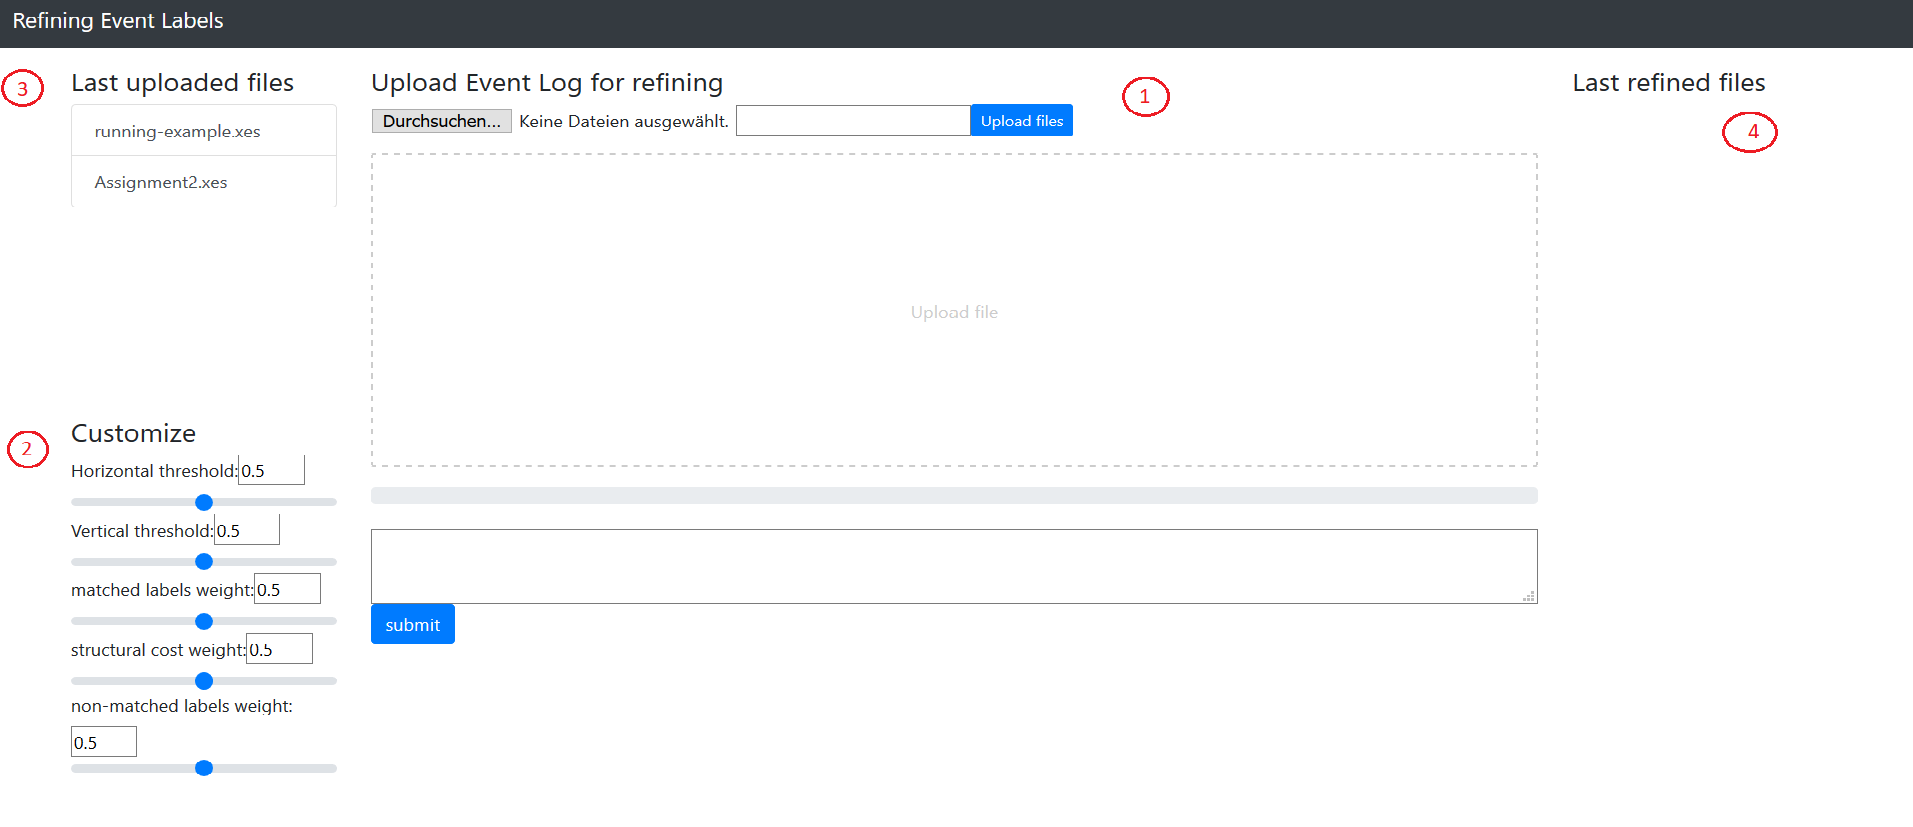
\includegraphics[scale=0.33]{startpage.png}
\caption{Overview of the start page with the different parts marked in red numbers}
\end{figure}

\subsection{Upload Event Log for refining}

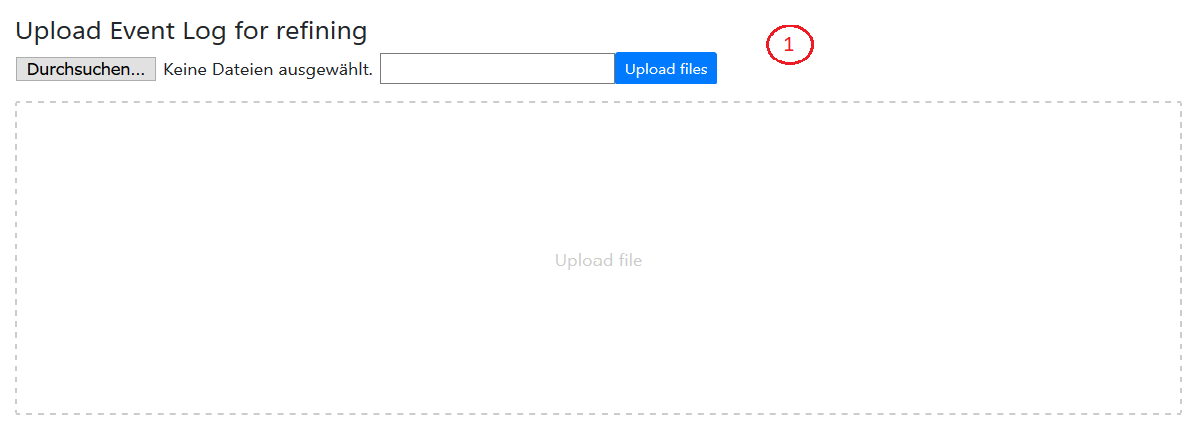
\includegraphics[scale=0.5]{uploadEventLog.png}

In this part of the start page, an event log can be uploaded. In order to do so, the user can either directly type in a path to a file and press the "Upload files" button, or he can use the "Search" button to search local files on his PC or drag a file into the big box with "Upload file" written in it. 
Afterwards, he has to press the "Upload files" button in order to upload the selected file. 

In order to successfully upload a file, this file has to be in XES or CSV format, otherwise an error will occur. 



\subsection{Customize}

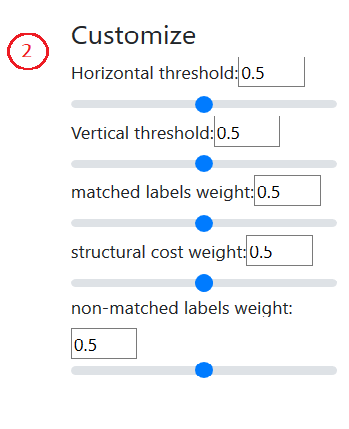
\includegraphics[scale=0.6]{customize.png}

In this section, the user can adjust the thresholds in order to fit his needs. 
To do so, he can either adjust them using the provided slide control or by typing them manually. 
The thresholds the user can adjust are the horizontal threshold, the vertical threshold, the weight structure, the weight for matched pairs of activities and the weight for not matched pairs of activities. 
All of the thresholds and weights have to be in the range from 0 to 1.
By default, all values are set to 0.5.

\subsection{Last uploaded files}

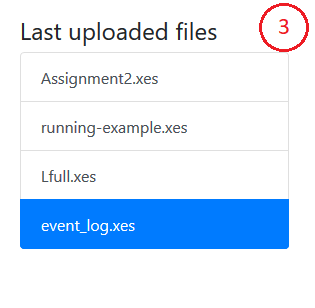
\includegraphics[scale=0.6]{lastUploadedFiles.png}

In this part of the start page, the user can see up to five of his last uploaded files. 
These files are not refined yet.
By clicking on them, he can select them and apply the refinement algorithm on them.

\subsection{Last refined files}

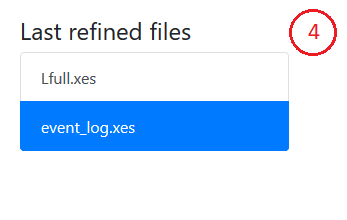
\includegraphics[scale=0.6]{lastRefinedFiles.png}

In this part of the start page, the user can see up to five of his last refined files. 
These files are already refined. 
By clicking on them, the user can download them.
The downloaded file has XES format and can be further used as input to process discovery algorithms.

\subsection{Candidate Labels}

\includegraphics[scale=0.5]{candidateLabels.png}

In this section, the user provides the algorithm with the candidate labels that should be subject to possible refinements. 
To do so, he enters the labels into the white box. 
The format should be: $label_1$,$label_2$,...,$label_n$ and the order of the labels does not matter.
After entering the candidate labels, the user can click on the "submit" button, so that the refinement algorithm will be run using the current thresholds, the chosen file and the provided candidate labels.
The fresh labels have the form $labelx.y$ with $x,y$ natural numbers.
Here $x$ identifies the refinement made in the horizontal refinement part of the algorithm, whereas $y$ identifies the refinement made in the vertical refinement part. 
If no labels are given or the given labels do not appear in the log, the refined log will be identical with the original one.

\section{Installation}

In order to use the web service, the folder refiningEventLabels has to be downloaded from the \href{https://github.com/NicoleVentsch/Refining-Event-Labels}{GitHub repository}. In this folder, the user can also find the code documentation in html format under $refiningEventLabels/lib/$ $documentation/_build/html/index.html$. 

After downloading the folder, Flask has to be installed. This can be done using the command:

\begin{lstlisting}
	pip install Flask 
\end{lstlisting}

Further information on how to install Flask can be found \href{http://flask.pocoo.org/docs/1.0/installation/}{here}. After opening a command prompt in the refiningEventLabels folder, the user needs to tell the terminal the application to work with by exporting the FLASK\_APP environment variable. This can be done using Windows by entering the following command:

\begin{lstlisting}
	C:\path\to\refiningEventLabels>set FLASK_APP=index.py
\end{lstlisting}
 
On Linux, the following command is needed:

\begin{lstlisting}
	 $ export FLASK_APP=index.py
\end{lstlisting}

More information on that can be found \href{http://flask.pocoo.org/docs/1.0/quickstart/}{here}.

\medskip

Now, the user can run Flask using the command:
\begin{lstlisting}
	 flask run
\end{lstlisting}

The output of this command will look like the following:


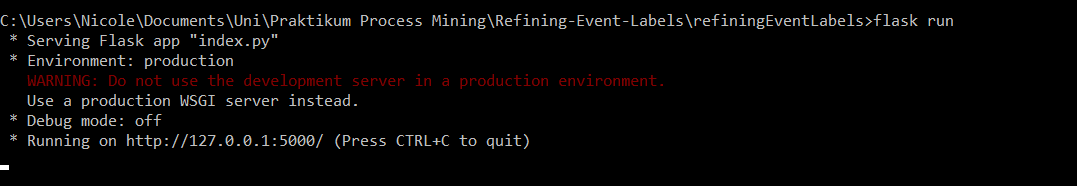
\includegraphics[scale=0.7]{Flask.png}


In the output, it is stated where the server is running, in this example on $http://127.0.0.1:5000/$. When typing this into a browser, the user will get to the start page of our web service and can then use it following the instructions found in section 2. 


\section{Technical background}

\subsection{Frontend}
The webapplication is optimized for Google Chrome (Version 65) and Mozilla Firefox (Version 60). 
The application has not been tested for Internet Explorer or other browser versions, so some parts may not work properly 
or the webinterface differs from the pictures. In order to access the API it is necessary to interpret the JSON object correctly.


\subsection{Backend}
The application backend can be executed on an Windows and Linux application server. 
This requires a Python version later than 3.6 and a Flask version later than 1.0. The index.py file in the application root dir indicates the 
entry point for the webapplication.

\section{Glossary}
In this section we give some brief description of the basic concepts used in the approach.
\medskip

\textbf{-task}\\
This is a synonym for the word event.
A task/event is unique in the log and it represents the recording of some action happening on a particular time.
We usually identify an event by the activity name assigned to it.
Many events (usually) have the same activity name describing "what" happened.
\medskip

\textbf{-label}\\
The labels stand for the activity names.
An event label is equal to the activity name of that event.
\medskip

\textbf{-label refinement}\\
By refining a label, we assign to it an other fresh label.
By definition of a refining function, two distinct labels do not get assigned the same new label.
\medskip

\textbf{-relabel}\\
A synonym for assigning a new name to a label.
\medskip

\textbf{-horizontal threshold}\\
This threshold is important in the horizontal refinement part of the algorithm.
For all pairs of traces in the log, we measure a value to capture the similarity (or dissimilarity) between them.
Traces are considered similar if this value is under the horizontal threshold.
The smaller the horizontal threshold, the more refinements take place.
\medskip

\textbf{-vertical threshold}\\
This threshold is important in the vertical refinement part of the algorithm.
In a set of traces which were considered similar in the horizontal refinement part of the algorithm, the same label may still appear many times.
By adjusting the vertical thresholds one affects the strictness of the refinement computed on these labels.
A lower threshold may induce more refinements.
\medskip

\textbf{-matched labels weight}\\
If a pair of events appears in a mapping, this weight denotes the importance we give to the dissimilarity these two events have in the set of their predecessor and successor labels.
\medskip

\textbf{-structural cost weight}\\
If a pair of events appears in a mapping, this weight denotes the importance we give to the dissimilarity these two events have in the positions they appear in the respective traces.
\medskip

\textbf{-non-matched labels weight}\\
For an event not appearing in a mapping, the cost of the mapping regarding the event is increased by the product of this weight with the number of predecessors and successors of this event.
\medskip


\section{Further improvements}
In this section we give some recommendations on how the algorithm can be adjusted or improved.
\medskip

$\bullet$
Instead of feeding the set of all variants to the refinement steps, one could remove those variants that do not contain any candidate labels.
This does not change the logic behind the approach.
However, in the case that the mapping with the maximal cost is one between two filtered variants, the normalized weights of the graph are going to be affected.
One can still obtain the same refined logs, but the corresponding thresholds yielding them would be slightly different.
\medskip

$\bullet$
In our implementation, we compute the context of each event by looking at the set of all its predecessors and successors.
One can change this to consider only the neighbors with maximal distance $k$ for some arbitrary $k$.
Moreover, one could add this parameter to the other Custom parameters, so that a user that has a good domain knowledge regarding his event log can determine the scope $k$.
\medskip

$\bullet$
For event logs containing a high number of trace variants or have long trace lengths which contain candidate labels, the algorithm has a long runtime.
This is due to the fact that in our implementation we calculate the costs of all the mappings between all pairs of traces and then pick the best one.
The calculation of the mappings can be further improved in a way that not all mappings are considered, but the difference in the results is negligible.

%\addcontentsline{toc}{chapter}{\textbf{References}}
%\end{flushleft}
%\bibliography{uw-ethesis}
% Tip 5: You can create multiple .bib files to organize your references. 
% Just list them all in the \bibliogaphy command, separated by commas (no spaces).

% The following statement causes the specified references to be added to the bibliography% even if they were not 
% cited in the text. The asterisk is a wildcard that causes all entries in the bibliographic database to be included (optional).



\begin{thebibliography}{5}
\bibitem{paper}
Lu, Xixi, et al. "Handling duplicated tasks in process discovery by refining event labels." International Conference on Business Process Management. Springer, Cham, 2016.

\bibitem{}
La Rosa M., Loos P., Pastor O. (eds) Business Process Management, BPM 2016, Lecture Notes in Computer Science, vol 9850. Springer, Cham, 2016.






\end{thebibliography}










\end{document}
